%
% fourier.tex -- oszillationsphänomene insbesondere Milankowitsch-Zyklern
%
% (c) 2018 Prof Dr Andreas Müller, Hochschule Rapperswil
%
\chapter{Fourier-Analysis\label{chapter:fourier}}
\lhead{Fourier-Analysis}
\rhead{ }
Im Kapitel~\ref{chapter:wetter und klima} wurde gezeigt, dass einige der
Einflüsse
auf das Klimasystem periodisch sind mit einer Periode, die vergleichbar
oder grösser ist als die bei der Definition des Begriffes Klima üblicherweise
verwendeten Mittelungszeitspanne.
Diese Anregungen führen daher zu periodischen Klimaschwankungen.
Die Fourier-Analysis ermögilcht, solche periodischen Einflüsse in
einem Signal zu erkennen und sie von anderen Phänomenen zu trennen.

%
% periodisch.tex -- periodische Funktionen
%
% (c) 2018 Prof Dr Andreas Müller, Hochschule Rapperswil
%
\section{Periodische Funktionen}


%
% fourierkoef.tex -- Bestimmung der Fourier-Koeffizienten
%
% (c) 2018 Prof Dr Andreas Müller, Hochschule Rapperswil
%
\section{Fourier-Koeffizienten}
Bestimmen wir die Fourierkoeffizienten für ein trigonometrisches Polynom
der Form
\begin{equation}
f(t)
=
a_0 + \sum_{k=1}^{n-1} a_k\cos kt + \sum_{k=1}^{n-1} b_k\sin kt + a_n\cos nt,
\label{skript:fourier:ansatz}
\end{equation}
so dass die Werte
\begin{equation}
y_j \quad\text{zu den Zeitpunkten}\quad t_j=2\pi\frac{j}{n},\qquad 1\le j\le N
\label{skript:fourier:gleichungen}
\end{equation}
möglichst genau die Funktionswerte $f(t_j)$ reproduzieren.
Im Ansatz~\eqref{skript:fourier:ansatz} finden wir $2n$ zu bestimmende 
Koeffizienten, in \eqref{skript:fourier:gleichungen} finden wir dagegen
genau $N$ Gleichungen, mit denen wir die Koeffizienten bestimmen könnten.
Für $N>2n$ haben wir also zu viele Daten, für $N<2n$ reichen die Datenpunkte
nicht, die Koeffizienten zu bestimmen.
Im optimalen Fall, für $N=2n$ sollte es möglich sein, die Koeffizienten so
zu bestimmen, dass die Funktionswerte $y_j$ exakt reproduziert werden.

\subsection{Least Squares}
Für $N>2n$ können wir nicht erwarten, dass der Ansatz die Daten
exakt reproduzieren kann, wir müssen uns also mit einer
Näherungslösung begnügen.
Wir verlangen stattdessen, dass der Fehler der Lösung möglichst gering
wird, dass also
\[
L=L(a_0,a_1,\dots,a_n,b_1,\dots,b_{n-1})= \sum_{j=1}^N (y_j - f(t_j))^2
\]
möglichst klein wird.

Die Grösse $L$ wird minimal, wenn alle Ableitungen nach den Koeffizienten
verschwinden:
\[
\frac{\partial L}{\partial a_0}=0,
\qquad
\frac{\partial L}{\partial a_l}=0, \;{1\le l\le n}
\qquad
\frac{\partial L}{\partial b_l}=0, \;{1\le l\le n-1}
\]
Wir berechnen die Ableitungen:
\begin{align*}
\frac{\partial L}{\partial a_0}
&=
-2 \sum_{j=1}^N (y_j-f(t_j))\cdot \frac{\partial f}{\partial a_0}(t_j)=0
&&
\\
\frac{\partial L}{\partial a_l}
&=
-2 \sum_{j=1}^N (y_j-f(t_j))\cdot \frac{\partial f}{\partial a_l}(t_j)=0
&k&=1,\dots,n
\\
\frac{\partial L}{\partial b_l}
&=
-2 \sum_{j=1}^N (y_j-f(t_j))\cdot \frac{\partial f}{\partial b_l}(t_j)=0
&k&=1,\dots,n-1
\end{align*}
Man beachte, dass der erste Klammerausdruck in der Summe die Koeffizienten
$a_0$, $a_k$ und $b_k$ nur linear enthält.
Die Funktion $f$ enthält die Koeffizienten ebenfalls nur linear, so
dass die Ableitungsterme die Koeffizienten nicht mehr enthalten werden.
Tatsächlich ergibt die Berechnung der Ableitungen
\begin{align*}
\frac{\partial f}{\partial a_0}(t_j)
&=
1
&&
\\
\frac{\partial f}{\partial a_l}(t_j)
&=
\cos lt_j
&l&=1,\dots,n
\\
\frac{\partial f}{\partial b_l}(t_j)
&=
\sin lt_j
&l&=1,\dots,n-1
\end{align*}
Die Gleichungen, die wir lösen müssen, sind also
\begin{equation}
\begin{aligned}
0&=
\sum_{j=1}^N
\biggl(
y_j - a_0 - \sum_{k=1}^n a_k\cos kt_j \sum_{k=1}^{n-1} b_k\sin kt_j
\biggl)
\\
&=
\sum_{j=1}^N y_j
-Na_0
-\sum_{k=1}^n a_k \sum_{j=1}^N\cos kt_j
-\sum_{k=1}^{n-1} b_k \sum_{j=1}^N\sin kt_j,
\\
0&=
\sum_{j=1}^N
\biggl(
y_j - a_0 - \sum_{k=1}^n a_k\cos kt_j \sum_{k=1}^{n-1} b_k\sin kt_j
\biggl) \cos lt_j
\\
&=
\sum_{j=1}^N y_j \cos lt_j
-a_0\sum_{j=1}^N \cos lt_j
-\sum_{k=1}^n a_k \sum_{j=1}^N\cos kt_j\cos lt_j
-\sum_{k=1}^{n-1} b_k \sum_{j=1}^N\sin kt_j\cos lt_j,
\\
0
&=
\sum_{j=1}^N
\biggl(
y_j - a_0 - \sum_{k=1}^n a_k\cos kt_j \sum_{k=1}^{n-1} b_k\sin kt_j
\biggl) \sin lt_j
\\
&=
\sum_{j=1}^N y_j \sin lt_j
-a_0\sum_{j=1}^N \sin lt_j
-\sum_{k=1}^n a_k \sum_{j=1}^N\cos kt_j\sin lt_j
-\sum_{k=1}^{n-1} b_k \sum_{j=1}^N\sin kt_j\sin lt_j.
\end{aligned}
\label{skript:fourier:gl2}
\end{equation}
Hier haben wir die Faktoren $-2$ ebenfalls weggelassen.

\subsection{Trigonometrische Summen}
In den Gleichungen~\eqref{skript:fourier:gl2} treten trigonometrische Summen
der Form
\begin{equation}
\sum_{j=1}^N \cos kt_j
\qquad
\text{oder}
\qquad
\sum_{j=1}^N \sin kt_j,
\label{skript:fourier:trigosum}
\end{equation}
der Summen von Produkten wie
\begin{equation}
\sum_{j=1}^N \cos kt_j\cos lt_j,\quad
\sum_{j=1}^N \cos kt_j\sin lt_j
\quad
\text{oder}
\quad
\sum_{j=1}^N \sin kt_j\sin lt_j
\label{fourier:produkte}
\end{equation}
auf.
In diesem Abschnitt sollen diese Summen mit Hilfe einer geometrischen
Überlegung berechnet werden.

Wir befassen uns zunächst mit Summen der Form
\label{skript:fourier:trigosum} und beweisen den folgenden Satz.

\begin{figure}
\centering
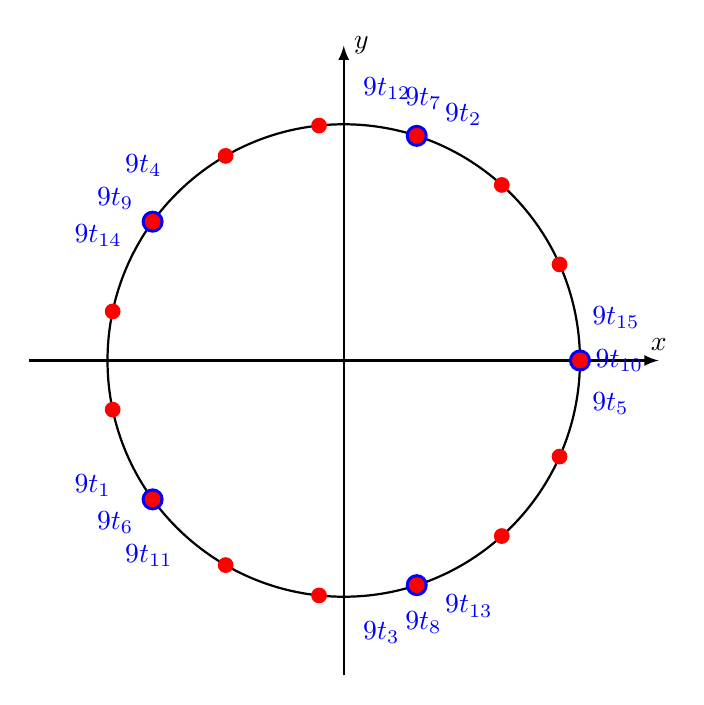
\begin{tikzpicture}[>=latex,thick]
\draw (0,0) circle[radius=3cm];
\draw[->] (-4,0)--(4,0) coordinate[label={$x$}];
\draw[->] (0,-4)--(0,4) coordinate[label={right:$y$}];
\foreach \j in {1,...,5}{
	\fill[color=blue] ({3 * cos(360 * \j/5)},{3 * sin(360 * \j/5)})
		circle[radius=0.14];
}
\def\N{15}
\foreach \j in {1,...,\N}{
	\fill[color=red] ({3 * cos(360 * \j/\N)},{3 * sin(360 * \j/\N})
		circle[radius=0.1];
}
\def\k{9}
\pgfmathparse{\k*360/\N}
\xdef\a{\pgfmathresult}
\def\j{1}
\def\r{0.5}
\pgfmathparse{\j*\a-9}\xdef\aa{\pgfmathresult}
\node[color=blue] at ({3*cos(\aa)},{3*sin(\aa)})
	[shift={({\r*cos(\aa)},{\r*sin(\aa)})}] {$9t_{1\phantom{0}}$};
\def\j{2}
\pgfmathparse{\j*\a-9}\xdef\aa{\pgfmathresult}
\node[color=blue] at ({3*cos(\aa)},{3*sin(\aa)})
	[shift={({\r*cos(\aa)},{\r*sin(\aa)})}] {$9t_{2\phantom{0}}$};
\def\j{3}
\pgfmathparse{\j*\a-9}\xdef\aa{\pgfmathresult}
\node[color=blue] at ({3*cos(\aa)},{3*sin(\aa)})
	[shift={({\r*cos(\aa)},{\r*sin(\aa)})}] {$9t_{3\phantom{0}}$};
\def\j{4}
\pgfmathparse{\j*\a-9}\xdef\aa{\pgfmathresult}
\node[color=blue] at ({3*cos(\aa)},{3*sin(\aa)})
	[shift={({\r*cos(\aa)},{\r*sin(\aa)})}] {$9t_{4\phantom{0}}$};
\def\j{5}
\pgfmathparse{\j*\a-9}\xdef\aa{\pgfmathresult}
\node[color=blue] at ({3*cos(\aa)},{3*sin(\aa)})
	[shift={({\r*cos(\aa)},{\r*sin(\aa)})}] {$9t_{5\phantom{0}}$};
\def\j{6}
\pgfmathparse{\j*\a}\xdef\aa{\pgfmathresult}
\node[color=blue] at ({3*cos(\aa)},{3*sin(\aa)})
	[shift={({\r*cos(\aa)},{\r*sin(\aa)})}] {$9t_{6\phantom{0}}$};
\def\j{7}
\pgfmathparse{\j*\a}\xdef\aa{\pgfmathresult}
\node[color=blue] at ({3*cos(\aa)},{3*sin(\aa)})
	[shift={({\r*cos(\aa)},{\r*sin(\aa)})}] {$9t_{7\phantom{0}}$};
\def\j{8}
\pgfmathparse{\j*\a}\xdef\aa{\pgfmathresult}
\node[color=blue] at ({3*cos(\aa)},{3*sin(\aa)})
	[shift={({\r*cos(\aa)},{\r*sin(\aa)})}] {$9t_{8\phantom{0}}$};
\def\j{9}
\pgfmathparse{\j*\a}\xdef\aa{\pgfmathresult}
\node[color=blue] at ({3*cos(\aa)},{3*sin(\aa)})
	[shift={({\r*cos(\aa)},{\r*sin(\aa)})}] {$9t_{9\phantom{0}}$};
\def\j{10}
\pgfmathparse{\j*\a}\xdef\aa{\pgfmathresult}
\node[color=blue] at ({3*cos(\aa)},{3*sin(\aa)})
	[shift={({\r*cos(\aa)},{\r*sin(\aa)})}] {$9t_{10}$};
\def\j{11}
\pgfmathparse{\j*\a+9}\xdef\aa{\pgfmathresult}
\node[color=blue] at ({3*cos(\aa)},{3*sin(\aa)})
	[shift={({\r*cos(\aa)},{\r*sin(\aa)})}] {$9t_{11}$};
\def\j{12}
\pgfmathparse{\j*\a+9}\xdef\aa{\pgfmathresult}
\node[color=blue] at ({3*cos(\aa)},{3*sin(\aa)})
	[shift={({\r*cos(\aa)},{\r*sin(\aa)})}] {$9t_{12}$};
\def\j{13}
\pgfmathparse{\j*\a+9}\xdef\aa{\pgfmathresult}
\node[color=blue] at ({3*cos(\aa)},{3*sin(\aa)})
	[shift={({\r*cos(\aa)},{\r*sin(\aa)})}] {$9t_{13}$};
\def\j{14}
\pgfmathparse{\j*\a+9}\xdef\aa{\pgfmathresult}
\node[color=blue] at ({3*cos(\aa)},{3*sin(\aa)})
	[shift={({\r*cos(\aa)},{\r*sin(\aa)})}] {$9t_{14}$};
\def\j{15}
\pgfmathparse{\j*\a+9}\xdef\aa{\pgfmathresult}
\node[color=blue] at ({3*cos(\aa)},{3*sin(\aa)})
	[shift={({\r*cos(\aa)},{\r*sin(\aa)})}] {$9t_{15}$};

\end{tikzpicture}
\caption{Verteilung der Punkte $(\cos t_j, \sin t_j)$  auf dem Einheitskreis 
in rot.
Die Punkte $(\cos kt_j,\sin kt_j)$ für $k=9$ bilden eine Teilmenge, die
blau dargestellt ist.
Jeder blaue Punkt wird genau dreimal besucht, sie bilden ein gleichseitiges
Fünfeck mit den Punkten $(\cos 3t_j,\sin 3t_j)$ als Ecken.
Deren Schwerpunkt ist wieder der Nullpunkt
\label{fourier:einheitskreis}
}
\end{figure}

\begin{satz}
Für beliebige ganze Zahlen $l$, $0\le l\le n$, gilt
\begin{equation*}
\begin{aligned}
\sum_{j=1}^N \cos lt_j
&=
\begin{cases}
N&\qquad l=0\\
0&\qquad\text{sonst}
\end{cases}
\\
\sum_{j=1}^N \sin lt_j
&=0
\end{aligned}
\end{equation*}
\end{satz}

\begin{proof}[Beweis]
Wir betrachten zunächst den Fall $l=0$.
In diesem Fall ist $\sin lt_j=0$ und $\cos lt_j=1$ und damit
\[
\sum_{j=1}^N \cos lt_j = N
\qquad\text{und}\qquad
\sum_{j=1}^N \sin lt_j = 0.
\]
Im Folgenden können wir daher annehmen, dass $l\ne 0$.

In Abbildung~\eqref{fourier:einheitskreis} kann man sehen, dass die Punkte
$(\cos t_j,\sin t_j)$ auf dem Einheitskreis ein regelmässiges Polygon
bilden.
Der Schwerpunkt des Polygons ist ganz offensichtlich der Mittelpunkt.
Daraus folgt
\[
\sum_{j=1}^N \cos t_j = 0
\qquad\text{und}\qquad
\sum_{j=1}^N \sin t_j = 0.
\]
Damit ist der Satz für den Fall $l=1$ bewiesen.

Für beliebiges $l\ne 0$ beobachten wir, dass die Punkte 
$(\cos lt_j,\sin lt_j)$ eine Teilmenge der Punkte $(\cos t_j, \sin t_j)$
sind.
Wenn $l$ und $N$ teilerfremd sind, sind die Mengen gleich.
Wenn $l$ und $N$ dagegen den grössten gemeinsamen Teiler $r$ haben, dann
ist die Menge der Punkte $(\cos rt_j,\sin rt_j)$, ein regelmässiges
Polygon mit $2\pi / rt_1$ Ecken.
Diese Situation ist in Abbildung~\ref{fourier:einheitskreis} mit den
blauen Punkten für den Fall $r=3=\operatorname{ggT}(9,15)$
illustriert.
Wie im Falle von $l=1$ folgt, dass der Schwerpunkt des Polygons der
Nullpunkt ist, und damit, dass
\begin{align*}
\sum_{j=1}^N \cos lt_j 
=
\sum_{j=1}^N \cos rt_j 
=
0,
\\
\sum_{j=1}^N \sin lt_j 
=
\sum_{j=1}^N \sin rt_j 
=
0.
\end{align*}
Damit ist alles gezeigt.
\end{proof}

In \eqref{fourier:produkte} werden die Summen von Produkten benötigt.
Mit üblichen trigonometrischen Umformungen kann man diese in Summen
von einfachen trigonometrischen Funktionen umwandeln.
Wir verwenden dazu die Formeln
\begin{align}
\cos\alpha\cos\beta
&=
\frac12(\cos(\alpha-\beta)+\cos(\alpha+\beta)),
\label{fourier:coscos}
\\
\sin\alpha\cos\beta
&=
\frac12(\sin(\alpha-\beta) + \sin(\alpha+\beta)),
\label{fourier:sincos}
\\
\sin\alpha\sin\beta
&=
\frac12(\cos(\alpha-\beta) + \cos(\alpha+\beta)).
\label{fourier:sinsin}
\end{align}
Damit können wir die Summen in \eqref{fourier:produkte} umwandeln:
\begin{align*}
\sum_{j=1}^N \cos kt_j\cos lt_j
&=
\sum_{j=1}^N \frac12(\cos (k-l)t_j +\cos(k+l)t_j)
\\
&=
\frac12\sum_{j=1}^N \cos (k-l)t_j
+ \frac12\underbrace{\sum_{j=1}^N\cos(k+l)t_j}_{\displaystyle=0}
\\
&=
\begin{cases}
\displaystyle\frac{N}2&\qquad k=l\\
0&\qquad\text{sonst}
\end{cases}
\\
\sum_{j=1}^N \sin kt_j \sin lt_j
&=
\sum_{j=1}^N \frac12(\cos(k-l)t_j +\cos(k+l)t_j)
\\
&=\frac12\sum_{j=1}^N \cos(k-l)t_j
+\frac12\underbrace{\sum_{j=1}^N \cos(k+l)t_j}_{\displaystyle=0}
\\
&=
\begin{cases}
\displaystyle\frac{N}2&\qquad k=l\\
0&\qquad\text{sonst}
\end{cases}
\\
\sum_{j=1}^N \sin kt_j \cos lt_j
&=
\sum_{j=1}^N \frac12(\sin(k-l)t_j +\sin(k+l)t_j)
\\
&=
\frac12\underbrace{\sum_{j=1}^N \sin(k-l)t_j}_{\displaystyle=0}
+
\frac12\underbrace{\sum_{j=1}^N \sin(k+l)t_j}_{\displaystyle=0}
=0.
\end{align*}
Damit haben wir den folgenden Satz bewiesen:

\begin{satz}
Für beliebige $k,l\in \mathbb N$ gilt
\begin{align*}
\sum_{j=1}^N
\cos kt_j \cos lt_j
&=
\begin{cases}
N                     &\qquad k=l=0\\
\displaystyle\frac{N}2&\qquad k=l > 0\\
0                     &\qquad\text{sonst}
\end{cases}
\\
\sum_{j=1}^N
\sin kt_j \sin l_j
&=
\begin{cases}
\displaystyle \frac{N}2&\qquad k=l\\
0                      &\qquad\text{sonst}
\end{cases}
\\
\sum_{j=1}^N
\sin kt_j \cos lt_j
&=
0
\end{align*}
\end{satz}
In den folgenden Abschnitten verwenden wir diese Formeln, um die
Koeffizienten $a_k$ und $b_k$ zu bestimmen.
Der Koeffizient $a_0$ muss wegen des ersten Falles im Satz gesondert
behandelt werden.

\subsection{Bestimmung von $a_0$}
In der Gleichung
\[
0
=
\sum_{j=1}^Ny_j
-Na_0
-\sum_{k=1}^na_k\underbrace{\sum_{j=1}^N\cos kt_j}_{\displaystyle=0}
-\sum_{k=1}^nb_k\underbrace{\sum_{j=1}^N\sin kt_j}_{\displaystyle=0}
\]
verschwinden die Summen über $j$ und es bleibt die Gleichung
\begin{align*}
0
&=
\sum_{j=1}^Ny_j
-Na_0
\\
\Rightarrow\qquad
a_0&=\frac1{N}\sum_{j=1}^N y_j.
\end{align*}

\subsection{Bestimmung von $a_k, k>0$}
Zur Bestimmung von $a_k$ mit $k>0$ müssen wir die Gleichung
\[
0
=
\sum_{j=1}^N y_j\cos lt_j
-
a_0\underbrace{\sum_{j=1}^N\cos lt_j}_{\displaystyle=0}
-\sum_{k=1}^na_k\sum_{j=1}^N\cos kt_j\cos lt_j
-\underbrace{\sum_{k=1}^nb_k\sum_{j=1}^N\sin kt_j\cos lt_j}_{\displaystyle=0}
\]
heranziehen.
Die zweite und vierte Summe verschwindet, so dass wir die
die Gleichung
\begin{align*}
0&=
\sum_{j=1}^N y_j\cos lt_j
-\sum_{k=1}^na_k\sum_{j=1}^N\cos kt_j\cos lt_j
\end{align*}
erhalten.
Die innere Summe über $j$ verschwindet für alle Werte von $k$ ausser
für $k=l$, in diesem Fall ist sie $N/2$. 
Damit können wir nach $a_k$ auflösen:
\begin{align*}
0&=
\sum_{j=1}^N y_j\cos lt_j
-a_l\frac{N}2
\\
\Rightarrow\qquad 
a_l &= \frac{2}{N}\sum_{j=1}^Ny_j\cos lt_j.
\end{align*}


\subsection{Bestimmung von $b_k$}
Zur Bestimmung von $b_k$ müssen wir die Gleichung
\[
0=\sum_{j=1}^N y_j\sin lt_j 
-a_0\sum_{j=1}^N \sin lt_j
-\sum_{k=1}^na_k\sum_{j=1}^N\cos kt_j\sin lt_j
-\sum_{k=1}^nb_k\sum_{j=1}^N\sin kt_j\sin lt_j
\]
heranziehen.
Die zweite und die dritte Summe verschwindet und in der letzten Summe
verschwinden alle Terme ausser der Term mit $k=l$, für den die
innere Summe den Wert $N/2$ hat.
Damit wird die Gleichung vereinfacht zu
\begin{align*}
0
&=
\sum_{j=1}^Ny_j\sin lt_j - b_l\frac{N}2
\\
\Rightarrow\qquad
b_l
&=
\frac{2}{N}\sum_{j=1}^Ny_j\sin lt_j.
\end{align*}


%
% vektorgeometrie.tex
%
% (c) 2018 Prof Dr Andreas Müller, Hochschule Rapperswil
%
\section{Vektorgeometrische Interpretation}
\rhead{Vektorschreibweise}
Die bisherigen rein analytischen Betrachtungen verdecken den geometrischen
Gehalt der bisher entwickelten Theorie.
In diesem Abschnitt soll daher zunächst eine vektorielle Darstellung
aufgebaut, die dann erlauben soll, einerseits die Formeln für die 
Fourierkoeffizienten geometrisch zu verstehen und andererseits auf
komplexere Situationen zu verallgemeinern.

\subsection{Vektoren}
Die Operationen zur Bestimmung der Fourier-Koeffizienten können in 
vektorieller Schreibweise etwas übersichtlicher dargestellt werden.
Zunächst fassen wir die Funktionswerte $y_j$ in einem Vektor zusamen.
\begin{equation}
y = \begin{pmatrix}y_1\\\vdots\\y_N\end{pmatrix}
\end{equation}
Zur Berechnung der Fourier-Koeffizienten brauchen wir auch noch die
Werte der trigonometrischen Funktionen zu den Zeiten $t_j$, die wir
ebenfalls als Vektoren
\begin{align*}
c_0&=\begin{pmatrix}0\\\vdots\\0\end{pmatrix},
&
c_k&=\begin{pmatrix}\cos kt_1\\\vdots\\\cos kt_N\end{pmatrix},\;(k=1,\dots,n)
&&\text{und}
&
s_k&=\begin{pmatrix}\sin kt_1\\\vdots\\\sin kt_N\end{pmatrix},\;(k=1,\dots,n-1)
\end{align*}
schreiben.
Die Fourier-Koeffizienten können jetzt als Skalarprodukte geschrieben werden:
\begin{align*}
a_0 &=\frac1N c_0\cdot y,&
a_k &=\frac2N c_k\cdot y,\;(k=1,\dots,n),&
b_k &=\frac2N s_k\cdot y,\;(k=1,\dots,n-1).
\end{align*}

\subsubsection{Rekonstruktion der Funktion}
Auch die Darstellung der Funktion kann man wieder als Skalarprodukt schreiben.
Dazu schreiben wir die Fourier-Koeffizienten und die Werte der
trigonometrischen Funtionen also Vektoren
\begin{align*}
a
&=
\begin{pmatrix}
a_0\mathstrut\\
a_1\mathstrut\\
b_1\mathstrut\\
a_2\mathstrut\\
b_2\mathstrut\\
\vdots\\
b_{n-1}\mathstrut\\
a_n\mathstrut
\end{pmatrix}
&&\text{und}
&
e(t)
&=
\begin{pmatrix}
1\\
\cos t\\
\sin t\\
\cos2t\\
\sin2t\\
\vdots\\
\sin(n-1)t\\
\cos nt
\end{pmatrix}.
\end{align*}
Damit wird 
\[
p(t) = a\cdot e(t)
\]

\subsubsection{Orthogonalität}
Die Aussagen von Satz~\ref{skript:fourier:orthogonalitaet1}
lassen sich jetzt in geometrische Form fassen.
\begin{satz}
Es gilt
\begin{align*}
c_k\cdot c_l
&=
\begin{cases}
N&\qquad k=l=0\\
\displaystyle\frac{N}2&\qquad k=l>0\\
0&\qquad\text{sonst}
\end{cases}
\\
s_k\cdot s_l
&=
\begin{cases}
\displaystyle\frac{N}2&\qquad k=l\\
0&\qquad\text{sonst}
\end{cases}
\\
c_k\cdot s_l
&=
0
\end{align*}
\label{skript:fourier:orthogonalitaet}
\end{satz}

\begin{proof}[Beweis]
Die genannten Skalarprodukte sind nichts anderes als die Summen in
Satz~\ref{skript:fourier:orthogonalitaet1}:
\begin{align*}
c_k\cdot c_l
&=
\sum_{j=1}^N \cos kt_j \cos lt_j
=
\begin{cases}
N&\qquad k=l=0\\
\displaystyle\frac{N}2&\qquad k=l>0\\
0&\qquad\text{sonst}
\end{cases}
\end{align*}
und analog für die anderen Skalarprodukte.
Die Aussage des Satzes ist daher nichts anders als eine geometrische
Umformulierung der Aussagen des
Satzes~\ref{skript:fourier:orthogonalitaet1}.
\end{proof}

\subsubsection{Die Identität von Parseval}
Die Relationen von
Satz~\ref{skript:fourier:orthogonalitaet1}
besagen, dass die Vektoren $c_k$ und $s_k$ orthogonal sind.
Wir wenden Sie auf das Skalarprodukt der Funktion $f$ mit sich selbst an.
\begin{align*}
f\cdot f
&=
a_0^2 c_0\,\cdot c_0
+
\sum_{k=1}^na_k^2 \,c_k\cdot c_k
+
\sum_{k=1}^{n-1} b_k^2\,s_k\cdot s_k
\\
&=
Na_0^2
+
\frac{N}2\sum_{k=1}^n a_k^2
+
\frac{N}2\sum_{k=1}^{n-1} b_k^2
=
\frac{N}2
\biggl(
2a_0^2
+
\sum_{k=1}^n a_k^2
+
\sum_{k=1}^{n-1} b_k^2
\biggr)
\end{align*}
Damit haben wir den folgenden Satz bewiesen:
\begin{satz}[Parseval]
\[
\|f\|^2
=
\sum_{j=1}^N y_j^2
=
\frac{N}2
\biggl(
2a_0^2
+
\sum_{k=1}^n a_k^2
+
\sum_{k=1}^{n-1} b_k^2
\biggr)
\]
\end{satz}

\subsubsection{$2\pi$-Periodische Funktionen auf $\mathbb R$}
Die eben vektoriell dargestellte Analyse diskreter periodischer Funktionen 
kann verallgemeinert werden auf die Analyse von Funktionen auf
anderen Definitionsgebieten.
Benötigt wird eine Familie von Basisfunktionen und ein Skalarprodukt
$\langle\;,\;\rangle$ derart, dass die Basisfunktionen $g_i$ bezüglich
dieses Skalarproduktes orthonormiert sind, dass also
\[
\langle g_i,g_j\rangle
=
\delta_{ij}
=
\begin{cases}
1&\qquad i=j\\
0&\qquad\text{sonst}.
\end{cases}
\]
Jede Linearkombination
\[
f = \sum_{i} \alpha_i g_i
\]
von Basisfunktionen kann ebenfalls mit dem Skalarprodukt rekonstruiert
werden.
Dazu berechnet man
\[
\langle g_i,f\rangle
=
\biggl\langle
g_i,\sum_j\alpha_jg_j
\biggr\rangle
=
\sum_j \langle g_i,\alpha_jg_j\rangle
=
\sum_j \alpha_j\delta_{ij}
=
\alpha_i.
\]
Das Skalarprodukt kann auch verwendet werden, um einen Abstand zwischen
Vektoren als
\[
\| f-g\|^2
=
\langle f-g,f-g\rangle
\]
zu definieren.

Dieselbe Situation lässt sich auch für $2\pi$-periodische Funktionen 
auf $\mathbb R$ herbeiführen.
Als Basisfunktionen kann man die Funktionen 
\begin{equation}
\frac{1}{\sqrt{2}},\; \cos kx,\; \sin lx\quad k>0
\label{fourier:basis}
\end{equation}
verwenden.
Das Skalarprodukt $\langle f,g\rangle$ muss linear in $f$ und $g$ sein.
Eine naheliegende Wahl ist
\[
\langle f, g\rangle
=
\frac{1}{\pi}\int_{-\pi}^{\pi} f(x)\,g(x)\,dx.
\]
Wir überprüfen, ob die Funktionen orthogonal sind:
\begin{align*}
\left\langle \frac1{\sqrt{2}},\frac1{\sqrt{2}}\right\rangle
&=
\frac1{\pi}
\int_{-\pi}^{\pi} \frac12\,dx
=
1
\\
\left\langle \frac1{\sqrt{2}},\cos kx\right\rangle
&=
\frac1{\pi}\int_{-\pi}^{\pi}
\frac1{\sqrt{2}}\cos kx
\,dx
=0
\\
\left\langle \frac1{\sqrt{2}},\sin kx\right\rangle
&=
\frac1{\pi}\int_{-\pi}^{\pi}
\frac1{\sqrt{2}}\sin kx
\,dx
=0
\\
\langle \cos kx,\cos lx\rangle
&=
\frac1{\pi}
\int_{-\pi}^\pi \cos kx\cos lx\,dx
\\
&=
\frac1{\pi}
\int_{-\pi}^\pi
\frac12\bigl(
\cos (k-l)x+\cos (k+l)x
\bigr)
\,dx
=
\begin{cases}
1&\qquad k=l\\
0&\qquad\text{sonst}
\end{cases}
\\
\langle \sin kx,\sin lx\rangle
&=
\frac1{\pi}
\int_{-\pi}^\pi \sin kx\,\sin lx\,dx
\\
&=
\frac1{\pi}
\int_{-\pi}^\pi
\frac12
\bigl(
\cos (k-l)x - \cos (k+l)x
\bigr)
\,dx
=
\begin{cases}
1&\qquad k=l\\
0&\qquad\text{sonst}
\end{cases}
\\
\langle \sin kx,\cos lx\rangle
&=
\frac1{\pi}
\int_{-\pi}^{\pi} 
\frac12\bigl(
\sin (k-l)x + \sin (k+l)x
\bigr)
\,dx
=0
\end{align*}
Zu einer $2\pi$-periodischen Funktion $f(x)$ kann man daher immer
die Koeffizienten
\begin{equation}
\begin{aligned}
\bar{a}_0&=\frac1{\pi\sqrt{2}}\int_{-\pi}f(x)\,dx
\\
a_k&=\frac1{\pi}\int_{-\pi}^\pi f(x)\cos kx\,dx
\\
b_k&=\frac1{\pi}\int_{-\pi}^\pi f(x)\sin kx\,dx
\end{aligned}
\label{fourier:normalekoeffizienten}
\end{equation}
berechnen.
Die Linearkombination
\begin{equation}
\tilde f(x)
=
\bar{a}_0\cdot\frac1{\sqrt{2}}
+ 
\sum_{k=1}^\infty (a_k\cos kx+b_k\sin kx)
\label{fourier:reihe}
\end{equation}
ist natürlich wieder eine $2\pi$-periodische Funktion.

Ist $f(x)$ eine Linearkombination von Funktionen~\eqref{fourier:basis},
dann sind nur endlich viele der Koeffizienten $\bar{a}_0$, $a_k$ und $b_k$
sind von $0$ verschieden und es gilt $f(x)=\tilde f(x)$, die Summe
\eqref{fourier:reihe} rekonstriert die Funktion $f(x)$ also exakt..

Für eine beliebige $2\pi$-periodische Funktion $f(x)$ ist die Funktion
$\tilde f(x)$ nach \eqref{fourier:reihe} im Allgemeinen eine unendliche
Reihe.
Die Reihe \eqref{fourier:reihe} heisst die Fourier-Reihe der Funktion 
$f(x)$.
\index{Fourier-Reihe}

In der Literatur wird $a_0$ meistens anders definiert, nämlich als
\[
a_0 = \frac1{\pi}\int_{-\pi}^{\pi} f(x)\,dx = \sqrt{2}\bar{a}_0
\qquad\Rightarrow\qquad
\bar{a}_0 = \frac{a_0}{\sqrt{2}}
\]
Der erste Term der Reihe~\eqref{fourier:basis} wird dann
\[
\bar{a}_0\cdot\frac1{\sqrt{2}}
=
\frac{a_0}{\sqrt{2}}\cdot\frac{1}{\sqrt{2}}
=
\frac{a_0}2
\]
und die Fourier-Reihe ist
\begin{equation}
\tilde f(x)
=
\frac{a_0}2
+
\sum_{k=1}^\infty (a_k\cos kx+b_k\sin kx).
\end{equation}

\subsection{Fourier-Transformation}
Die Fourier-Koeffizienten $a_k$ und $b_k$ hängen linear von den
Funktionswerten $y_j$ ab.
Der Vektor der Fourier-Koeffizienten muss daher der Bildvektor des
Vektors $\vec y$ der Funktionswerte unter einer linearen Transformation
sein.
In diesem Abschnitt soll zunächst diese diskrete Fourier-Transformation 
hergeleitet werden.
Anschliessend soll gezeigt werden, wie sich diese Eigenschaft auf 
periodische Funktionen und auf beliebige Funktionen auf $\mathbb R$
ausdehenen lässt.

\subsubsection{Diskrete Fourier-Transformation}
Die Berechnung der Fourier-Koeffizienten ist eine lineare Operation
mit der $N\times N$-Matrix:
\[
A
=
\begin{pmatrix}
c_0^t\\
c_1^t\\
s_1^t\\
\vdots\\
c_{n-1}^t\\
s_{n-1}^t\\
c_n^t
\end{pmatrix}
=
\begin{pmatrix}
1           &1           &\dots &1            \\
\cos t_1    &\cos t_2    &\dots &\cos t_N     \\
\sin t_1    &\sin t_2    &\dots &\sin t_N     \\
\cos 2t_1   &\cos 2t_2   &\dots &\cos 2t_N    \\
\sin 2t_1   &\sin 2t_2   &\dots &\sin 2t_N    \\
\vdots      &\vdots      &\ddots&\vdots       \\
\sin(n-1)t_1&\sin(n-1)t_2&\dots &\sin(n-1)t_N \\
\cos nt_1   &\cos nt_2   &\dots &\cos nt_N    
\end{pmatrix}
\]
Die Orthogonalitätsrelationen von
Satz~\ref{skript:fourier:orthogonalitaet}
können jetzt neu geschrieben werden:
\begin{align*}
AA^t
&=
\begin{pmatrix}
c_0\cdot c_0&
	c_0\cdot c_1&
		c_0\cdot s_1&
			\dots&
				c_0\cdot c_{n-1}&
					c_0\cdot s_{n-1}&
						c_0\cdot c_n\\
c_1\cdot c_0&
	c_1\cdot c_1&
		c_1\cdot s_1&
			\dots&
				c_1\cdot c_{n-1}&
					c_1\cdot s_{n-1}&
						c_1\cdot c_n\\
s_1\cdot c_0&
	s_1\cdot c_1&
		s_1\cdot s_1&
			\dots&
				s_1\cdot c_{n-1}&
					s_1\cdot s_{n-1}&
						s_1\cdot c_n\\
\vdots	&\vdots	&\vdots	&\ddots	&\vdots	&\vdots	&\vdots	\\
c_{n-1}\cdot c_0&
	c_{n-1}\cdot c_1&
		c_{n-1}\cdot s_1&
			\dots&
				c_{n-1}\cdot c_{n-1}&
					c_{n-1}\cdot s_{n-1}&
						c_{n-1}\cdot c_n\\
s_{n-1}\cdot c_0&
	s_{n-1}\cdot c_1&
		s_{n-1}\cdot s_1&
			\dots&
				s_{n-1}\cdot c_{n-1}&
					s_{n-1}\cdot s_{n-1}&
						s_{n-1}\cdot c_n\\
c_n\cdot c_0&
	c_n\cdot c_1&
		c_n\cdot s_1&
			\dots&
				c_n\cdot c_{n-1}&
					c_n\cdot s_{n-1}&
						c_n\cdot c_n\\
\end{pmatrix}
\\
&=
\begin{pmatrix}
N     &0        &0        &\dots    &0        &0        &0        \\
0     &\frac{N}2&0        &\dots    &0        &0        &0        \\
0     &0        &\frac{N}2&\dots    &0        &0        &0        \\
\vdots&\vdots   &\vdots   &\ddots   &\vdots   &\vdots   &\vdots   \\
0     &0        &0        &\dots    &\frac{N}2&0        &0        \\
0     &0        &0        &\dots    &0        &\frac{N}2&0        \\
0     &0        &0        &\dots    &0        &0        &\frac{N}2
\end{pmatrix}.
\end{align*}
Bis auf die Faktoren $N$ und $\frac{N}2$ auf der Diagonalen ist
${\cal F}{\cal F}^t$ 
eine Diagonalmatrix.
Wir können die Matrix zu einer Einheitsmatrix machen, indem wir 
sie mit der Diagonalmatrix
\begin{equation}
D
=
\begin{pmatrix}
\sqrt{\frac1N}&0&\dots&0\\
0&\sqrt{\frac{2}{N}}&\dots&0\\
\vdots&\vdots&\ddots&\vdots\\
0&0&\dots&\sqrt{\frac{2}{N}}
\end{pmatrix}
\end{equation}
multiplizieren.
Wir schreiben
\begin{align*}
{\cal F}
&=
D\, A
\end{align*}
Wir nennen $\cal F$ die {\em Fourier-Matrix}.
\index{Fourier-Matrix}%
Die Fourier-Matrix $\cal F$ ist orthogonal, es gilt
\[
{\cal F}{\cal F}^t
=
DAA^tD^t
=
DD^tAA^t
=
E,
\]
wobei wir im letzten Schritt $D^t$ mit $AA^t$ vertauschen durften,
weil beide Diagonalmatrizen sind und damit vertauschen.
Insbesondere erhält $\cal F$ das Skalarprodukt, womit wir natürlich
nur die Parseval-Identität anders formuliert haben.

\subsubsection{Fast Fourier Transform}


\subsubsection{Fourier-Transformation von $2\pi$-periodischen Funktionen}

\subsubsection{Fourier-Transformation von Funktionen auf $\mathbb R$}








\section*{Übungen}
\begin{uebungsaufgaben}
\item
Betrachten Sie die Differentialgleichung
\begin{equation}
\frac{dx}{dt}
=
x^4-4x^2-\lambda
\label{aufgabe301:gl}
\end{equation}
\begin{teilaufgaben}
\item
Finden Sie die Gleichgewichtslösungen und untersuchen Sie die 
Bifurkationen, die bei Veränderungen des Parameters $\lambda$
auftreten können.
\item
Welche Gleichgewichtslösung wird das System einnehmen, wenn der
Parameter $\lambda$ erst von $-1$ auf $1$ anwächst
und dann wieder auf $-1$ absinkt.
\end{teilaufgaben}

\begin{loesung}
\begin{figure}
\centering
\includegraphics{chapters/3/grad4.pdf}
\caption{Phasendiagramm der Differentialgleichung~\eqref{aufgabe301:gl}.
\label{aufgabe301:fig}}
\end{figure}
\begin{teilaufgaben}
\item
Die kritischen Punkte der Differentialgleichung~\eqref{aufgabe301:gl}
sind Nullstellen der Gleichung
\begin{equation}
x^4-4x^2-\lambda=0
\label{aufgabe301:gl}
\end{equation}
Dies ist eine quadratische Gleichung in $x^2$, die mit der Lösungsformel
für die quadratische Gleichung gelöst werden kann:
\[
x^2 = 2 \pm \sqrt{4+\lambda}.
\]
Diese Gleichung hat reelle Lösungen für $\lambda \ge -4$.
Für $\lambda \le 0$ ist die Quadratwurzel nicht grösser als $2$,
so dass die beiden Nullstellen positiv sind, es also vier verschiedene
Lösungen
\begin{equation}
x_{1,2,3,4} = \pm\sqrt{2\pm\sqrt{4+\lambda}}
\end{equation}
hat.
Für $\lambda >0$ hat die quadratische Gleichung eine negative Lösung
für $x^2$, die also nicht zu einer reellen Lösung der
Gleichung~\eqref{aufgabe301:gl} führen kann.
Nur aus der positive Lösung $2+\sqrt{4+\lambda}$ kann man eine
Gleichgweichslösung, nämlich
\[
x=\pm\sqrt{2+\sqrt{4+\lambda}}
\]
ableiten.
Für $\lambda < -4$ gibt es gar keine Gleichgewichtslösung.

Das Phasendiagramm in Abbildung~\ref{aufgabe301:fig} zeigt,
dass für $\lambda >0$ die obere Gleichgewichtslösung stabil ist,
untere dagegen instabil.
Für $-4\le\lambda\le 0$ sind die Gleichgewichtslösungen
\begin{align*}
&\sqrt{2+\sqrt{4+\lambda}}
&&\text{und}&
&-\sqrt{2-\sqrt{4+\lambda}}
\\
\intertext{stabil und die Gleichgewichtslösungen}
&-\sqrt{2+\sqrt{4+\lambda}}
&&\text{und}&
&\sqrt{2-\sqrt{4+\lambda}}
\end{align*}
instabil.

Bei $\lambda=-4$ finden gleichzeitig zwei Sattel-Knoten-Bifurkationen 
statt, bei $\lambda=0$ findet ein einfache Sattel-Knoten-Bifurkation
statt, jedoch in umgekehrter Richtung wie im Beispiel im Text.
\item
Beim Anwachsen des Parameters über den Punkt $\lambda=0$ springt die
Gleichgewichtslösung auf die stabile Lösung
\[
x(\lambda)=\sqrt{2+\sqrt{4+\lambda}}.
\]
Bei der anschliessenden Verringerung von $\lambda$ bleibt die 
Gleichgewichtslösung auf dem Ast $x(\lambda)$ der Kurve, da diese
alle stabil sind.
Unabhängig vom Ausgangszustand befindet sich das System am Ende des
beschriebenen Szenarios also immer in der Nähe der Gleichgewichtslösung
\[
x(-1)=\sqrt{2+\sqrt{3}}.
\qedhere
\]
\end{teilaufgaben}
\end{loesung}


\end{uebungsaufgaben}

